%%%%%%%%%%%%%%%%%%%%%%%%%%%HEADER%%%%%%%%%%%%%%%%%%%%%%%%%%%%%%
%%%%%%%%%%%%%%%%%%%%%%%%%%%HEADER%%%%%%%%%%%%%%%%%%%%%%%%%%%%%%
%%%%%%%%%%%%%%%%%%%%%%%%%%%HEADER%%%%%%%%%%%%%%%%%%%%%%%%%%%%%%
%Note: All the options like chapterprefix, pointednumbers, etc affect the way things are represented in the header of each page
\documentclass[a4paper,12pt,oneside,pointednumbers,numbers=noenddot,bibtotoc,bigheadings,liststotoc,chapterprefix=true]{scrbook}
% note that the expression "numbers=noenddot" remoes the dot after the number in figure captions
% for details see https://tex.stackexchange.com/questions/27250/remove-dot-after-number-in-figure-captions-while-keeping-the-dot-in-chapter-sect
\usepackage[utf8]{inputenc} %für Umlaute etc.
\usepackage[T1]{fontenc}
\usepackage[ngerman, english]{babel} %English titles (figure, table) und englische Silbentrennung
\usepackage{a4wide}
\usepackage{parskip} %see https://golatex.de/wiki/%5Cparskip to know what the package can do
\usepackage[pdftex]{color}
\usepackage{lmodern} \normalfont %to load T1lmr.fd  %weniger verpixelte Schrift; mehr Infos: http://www.namsu.de/Extra/pakete/Lmodern.html
%den genauen Trick für die untere Zeile kann ich hier nochmal nachlesen: http://tex.stackexchange.com/questions/22240/choosing-font-for-bold-small-caps-or-any-other-particular-familyseriesshape-c
\DeclareFontShape{T1}{lmr}{bx}{sc} { <-> ssub * cmr/bx/sc }{} 
\usepackage{a4} %anscheinend besser hier die Formatierung a4 wählen als als Option von documentclass
\usepackage[bookmarks]{hyperref}
%\usepackage{fancyhdr}
\usepackage[right]{eurosym}
% the below two lines of code are necessary to make sure that the numbering of figures starts at 1 and then proceeds in steps of 1 instead of floating point numbers etc.
\usepackage{chngcntr}
\counterwithout{figure}{chapter}
\counterwithout{table}{chapter}
% the below code allows the adjustment 

\usepackage{amsmath, amssymb, amstext} %für Mathematik
\usepackage{mathstyle} %mehr Infos: http://www.ctan.org/pkg/mathstyle
\usepackage{blindtext} %to be able to place blindtext at certain locations
\usepackage[left=40mm, right=40mm, top=50mm, bottom=30mm]{geometry}%Seitenränder anpassen
\usepackage[onehalfspacing]{setspace} %1.5 Zeilgenabstand
\usepackage[round, comma]{natbib} %für die Bibliographie
%all four of the below packages are included for table creation
\usepackage{booktabs} 
\usepackage{array}
\usepackage{multirow}
\usepackage{tabularx}
\usepackage{mathstyle} %mehr Infos: http://www.ctan.org/pkg/mathstyle
\usepackage[pdftex]{graphicx} %to include graphics
\usepackage{microtype} % makes pdf look better
\usepackage{booktabs}
%the below package allows the modification of the enumeration symbols
\usepackage{enumerate}% http://ctan.org/pkg/enumerate
\usepackage{dcolumn} % Ausrichtung nach Dezimalpunkt in Tabellen
\newcolumntype{.}{D{.}{.}{-1}}
\usepackage{setspace}
\pagestyle{headings}
% the below code is necessary to be able to customize the font of the Figure caption for figures
\usepackage{caption} % see https://www.namsu.de/Extra/pakete/Caption.html for more information!
\captionsetup[table]{font=footnotesize,labelfont=footnotesize,labelfont=bf, singlelinecheck = false, format=hang, justification=centering}
\captionsetup[figure]{font=footnotesize,labelfont=footnotesize,labelfont=bf, singlelinecheck = false, format=plain, justification=raggedright}%width=\dimexpr\textwidth-2cm\relax}
%\setlength{\textwidth}{15cm}
%\setlength{\textheight}{22.5cm}
%\setlength{\oddsidemargin}{1cm}
%\setlength{\evensidemargin}{0cm}
% \renewcommand{\baselinestretch}{1.2}
% \parskip1ex plus0.5ex minus0.5ex
%um die Überschriften im Inhaltsverzeichnis anzupassen
\usepackage{tocloft}
\renewcommand{\cftchapaftersnum}{.} %add period after the chapter number in ToC
% see https://tex.stackexchange.com/questions/411708/add-period-in-list-of-figures-list-of-tables
\renewcommand{\cftfigaftersnum}{.} %add period after figure number in list of figures
\renewcommand{\cfttabaftersnum}{.} %add period after table number in list of tables
\renewcommand\cftchapfont{\large\bfseries}%changes font and fontsize of chapters in toc
%\renewcommand\cftsecfont{\normalsize}
\renewcommand{\cfttoctitlefont}{\huge\bfseries}	%changes font of 'Content' header before toc
\renewcommand{\cftloftitlefont}{\huge\bfseries} %changes font of 'List of Figures'
\renewcommand{\cftlottitlefont}{\huge\bfseries} %changes font of 'List of Tables'
% the below commands move the beginning of toc, list of figures and list of tables further down 
% the page
\renewcommand\cftbeforetoctitleskip{2.7cm}
\renewcommand\cftbeforeloftitleskip{2.7cm}
\renewcommand\cftbeforelottitleskip{2.7cm}
%um die Überschriften im Text anzupassen
\usepackage{titlesec}
%der folgende Befehl ändert die Schriftart des "chapter"-Befehls
\titleformat{\chapter}{\large\bfseries\filright}{\Huge\thechapter.}{15pt}{\Huge}
\titleformat*{\section}{\Large\bfseries}
\titleformat*{\subsection}{\large\bfseries}
\titleformat*{\subsubsection}{\large\bfseries}
\titleformat*{\paragraph}{\small\bfseries}

%---------------------------------------------------------------------- Customizations ---------------------------------------------------------------------
%--------------------------------
%--------------------------------the entire below part is necessary to be able to include an abstract with the books document class
%--------------------------------
\usepackage{lipsum}
\newcommand\abstractname{Abstract}  %%% here
\makeatletter
\if@titlepage
  \newenvironment{abstract}{%
      \titlepage
      \null\vfil
      \@beginparpenalty\@lowpenalty
      \begin{center}%
        \bfseries \abstractname
        \@endparpenalty\@M
      \end{center}}%
     {\par\vfil\null\endtitlepage}
\else
  \newenvironment{abstract}{%
      \if@twocolumn
        \section*{\abstractname}%
      \else
        \small
        \begin{center}%
          {\bfseries \abstractname\vspace{-.5em}\vspace{\z@}}%
        \end{center}%
        \quotation
      \fi}
      {\if@twocolumn\else\endquotation\fi}
\fi
\makeatother

%--------------------------------
%--------------------------------the entire below part is necessary to be able to customize the header
%--------------------------------

\usepackage{fancyhdr} %Paket für Kopf- und Fußzeile laden
\setlength{\headheight}{15.2pt}
\pagestyle{fancy} %wir aktivieren unseren eigenen Seitenstil
%der folgende Befehl ändert die Schriftart im Header:
\renewcommand{\chaptermark}[1]{\markboth{\chaptername\  
\thechapter. \textit{#1}}{}}
\fancyhf{} %alle Kopf- und Fußzeilenfelder bereinigen
\fancyhead[R]{\thepage}
\fancyhead[L]{\rightmark}
\renewcommand{\headrulewidth}{0.4pt} %customizing obere Trennlinie

% a bunch of code to control the length of the headrule
% Length to control the \fancyheadoffset and the calculation of \headline
% simultaneously
\newlength\FHoffset
\setlength\FHoffset{0cm}

\addtolength\headwidth{2\FHoffset}

\fancyheadoffset{\FHoffset}

% these lengths will control the headrule trimming to the left and right 
\newlength\FHleft
\newlength\FHright

% here the trimmings are controlled by the user
\setlength\FHleft{0cm}
\setlength\FHright{0cm}

% The new definition of headrule that will take into acount the trimming(s)
\newbox\FHline
\setbox\FHline=\hbox{\hsize=\paperwidth%
  \hspace*{\FHleft}%
  \rule{\dimexpr\headwidth-\FHleft-\FHright\relax}{\headrulewidth}\hspace*{\FHright}%
}
\renewcommand\headrule{\vskip-.7\baselineskip\copy\FHline}
% above is a bunch of code to control the length of the headrule


%--------------------------------
%--------------------------------additional customizations
%--------------------------------
\setlength{\parindent}{0pt} %legt die Einrücktiefe der ersten Zeile für alle folgenden Absätze fest
\setlength{\abovecaptionskip}{-15pt plus 3pt minus 2pt} %modify vertical space between figure and caption
\renewcommand*{\paragraph}[1]{\subsubsection*{#1} \vspace{-3mm}} %mit diesem Befehl kann man ganz einfach
%PARAGRAPH eingeben und latex macht sofort eine subsubsection ohne Nummerierung usw draus
%customizations für Vektoren (dass sie bold dargestellt werden anstatt mit einem Vektorpfeil)
\let\oldhat\hat
\renewcommand{\vec}[1]{\boldsymbol{#1}}
\renewcommand{\hat}[1]{\oldhat{\boldsymbol{#1}}}

%%%%%%%%%%%%%%%%%%%%BEGINNING OF THE DOCUMENT%%%%%%%%%%%%%%%%%%%%%%%%
%%%%%%%%%%%%%%%%%%%%BEGINNING OF THE DOCUMENT%%%%%%%%%%%%%%%%%%%%%%%%
%%%%%%%%%%%%%%%%%%%%BEGINNING OF THE DOCUMENT%%%%%%%%%%%%%%%%%%%%%%%%
\begin{document}
%----------------------------------------------------------- Beginn Titelseite -------------------------------------------------------------------------------
%\changefont{ppl}{m}{n} %mit diesem Befehl kann global ganz leicht die Schriftart geändert werden
\newgeometry{left=30mm, right=30mm, top=0mm, bottom=0mm}
\begin{titlepage}
    \begin{center}
        \hspace*{-0.27\textwidth}
\includegraphics[width=1.419\textwidth, trim = 5mm 250mm 0mm 0mm, clip = TRUE]{logo.pdf}\hspace*{-0.3\textwidth}
        \quad \\[0mm]
        \newcommand{\HRule}{\rule{\linewidth}{0.3mm}} %Befehl zum Erstellen der Linie
        \HRule \\[-1mm]
        \Huge{\scshape\bfseries Uncertainty and Business Cycles} \\[-5mm]
        \HRule \\[2mm]
        \Large {\scshape\bfseries An Empirical Analysis using \\
                   Local Projections \\
                   (work in progress)} \\[10mm]
        \large Masterarbeit \\[20mm]
        \large zur Erlangung des akademischen Grades eines \\ Master of Science (M.Sc.)\\
                  in Applied Economics \\[10mm]
                  
        eingereicht bei Herrn\\
        Univ.-Prof. Dr. Johann Scharler \\[10mm]
        Institut für Wirtschaftstheorie, -politik und -geschichte\\
        Fakultät für Volkswirtschaft und Statistik\\
        Leopold-Franzens-Universität Innsbruck \\[10mm]
        von \\ Mag. Marcel A. Kropp \\[10mm]
        Innsbruck, Juli 2018
    \end{center}
\end{titlepage}
%----------------------------------------------------------- Ende Titelseite -------------------------------------------------------------------------------
\restoregeometry

%----------------------------------------------------------- Beginn Widmung Mum ---------------------------------------------------------------------
%Kurze Widmung an Mum.
\thispagestyle{empty} %bewirkt, dass die Striche oben wegfallen und, dass die Seitenzahl wegfällt.
\null\vspace{\stretch{1}}
    \begin{flushright}
       % \large \textit{To my Mum.}\\
    \end{flushright}
\vspace{\stretch{2}}\null
%----------------------------------------------------------- Ende Widmung Mum ------------------------------------------------------------------------


%----------------------------------------------------------- Beginn Widmung Alle ------------------------------------------------------------------------
\newpage
\pagestyle{empty} %bewirk, dass die Striche oben wegfallen und, dass die Seitenzahl wegfällt.
%What I have written five years ago still holds more than ever:\\
%My family has been my strongest support in all my life. I especially want to express my gratitude to my dear uncle Dr. med. Farshid Mavaddat, my cousins Dr. Paik Saber and Neisan Saber and my aunt Mahshid Mavaddat.\\
%Most of all I want to thank my Mum, Dorrie Mavaddat, who has always been there for me and supported and helped my in all my ventures. It is due to her that I stand where I am today.
%    \begin{flushright}
%         Innsbruck, July 2018\\
%    \end{flushright}
\pagestyle{headings}
%-------------------------------------------------------------- Ende Widmung Alle ------------------------------------------------------------------------

%\clearpage
%\setlength{\hoffset}{0mm}

%jetzt kommen die abstracts auf Englisch und Deutsch
\thispagestyle{empty} 
%\quad \\[2cm]
\selectlanguage{english}
\begin{abstract}
\blindtext
\end{abstract}

%\quad \\[10mm]
\begin{otherlanguage}{ngerman}
\begin{abstract}
\blindtext
\end{abstract}
\end{otherlanguage}


\restoregeometry

\thispagestyle{empty}
\pagestyle{fancy} %bewirkt, dass die Striche oben wieder dazukommen
\pagenumbering{roman} %bewirkt, dass LateX i, ii, usw zählt
\setcounter{page}{7} %und aber schon bei 7 anfängt zu zählen
%\renewcommand{\contentsname}{Table of Contents}
%\renewcommand{\cftdot}{\ensuremath{\ast}} %\ensuremath{\ast} does sth funny to the dots in the toc
\tableofcontents
\newpage
\listoffigures

\newpage
\listoftables

\newpage

%%%%%%%%%%%%%%%%%AB HIER BEGINNT DER INHALT DER ARBEIT%%%%%%%%%%%%%%%%%%%%%
%%%%%%%%%%%%%%%%%AB HIER BEGINNT DER INHALT DER ARBEIT%%%%%%%%%%%%%%%%%%%%%
%%%%%%%%%%%%%%%%%AB HIER BEGINNT DER INHALT DER ARBEIT%%%%%%%%%%%%%%%%%%%%%
\pagenumbering{arabic} %mit diesem Befehl wechseln wir auf 1, 2, 3, usw. zum zählen.
\chapter{Introduction}
% the below code making use of "begingroup" etc. is only necessary if I want to customize the font for a particular part of the thesis
%\begingroup
%\fontsize{10pt}{12pt}\selectfont
Similarly to how \citet{bloom:09} has mentioned that studying uncertainty is incredibly topical given the recent Brexit and Trump election outcomes (see \url{https://site.stanford.edu/2018/session-6}), I could start the introduction along similar lines.\footnote{The mentioned link is about a Summer Workshop related to 'Macroeconomics of Uncertainty and Volatility' in which Bloom also briefly mentions that the theoretical and empirical understanding of how uncertainty affects economies as a whole is still limited since macroeconomists only recently have started working on these issues from a more systematic basis. Still, he mentions about 14 recent papers on this topic (which are not yet posted online but which I could include into the literature review as well!)}.
\\
\\
Some notes to myself when reading through some of the articles:
\begin{itemize}  
	\item ``Real GDP has the virtue of being the broadest indicator of real economic activity. Its downside is that it is difficult to measure [...]. For this reason, we also consider two other indicators: industrial production and the unemployment rate. Industrial production has the benefit of being relatively straightforward to measure; unemployment has the benefit of being perhaps the closest to a purely cyclical indicator.'' (Romer \& Romer, p. 3092)
	\item Footnote 17 in \citet{romandrom:17}: ``The impulse response functions in Figure 4 are estimated using the Jordà local projection method. Figure C2 of online Appendix C shows that the results estimated using a conventional vector autoregression are virtually identical.'' --> should we include a comparison with Bloom's VAR?
	\item \citet[p. 3096]{romandrom:17}: ``To do this, we run the same regression as in equation (1), but with our new measure of financial distress as the dependent variable. Since by construction the response of distress to itself is one at t = 0, we only estimate the regression for horizons 1 to 10. This analysis shows that distress is very serially correlated, particularly at near horizons. This finding suggests that some of the near-term persistence we find in the negative aftermath of financial distress is likely due to persistence in distress itself. It is not necessarily that financial crises have long-lasting effects, but rather that crises themselves tend to last for a while. This possibility [...] is analyzed further in Section III.''
	\item \citet[p. 3097]{romandrom:17}: ``Given that our new series on financial distress differs in important ways from existing crisis chronologies, it is useful to compare our findings for the average aftermath of financial crises with those estimated using the other series.'' --> We can use this approach similarly by using various uncertainty measures in our regressions as alternative and compare the impulse-response functions.
	\item \citet[p. 3099]{romandrom:17}, \textit{Dealing with Heteroskedasticity}: ``The first issue is possible differences in the variance of the residuals across countries. Economic activity is typically much more volatile in the less developed countries in our sample (such as Greece and Turkey), and in the smaller countries. It is plausible to think that the variances of the residuals in equation (1) also vary systematically by country. \\
	--> Taking into account heteroskedasticity in the residuals has a substantial impact on the estimates. Though the time pattern of the decline in GDP is relatively unchanged, the maximum decline is reduced by about one-third.''
	\item \citet[p. 3010]{romandrom:17}: ``In a related exercise, we also consider alternatives to conventional standard errors. In addition to heteroskedasticity of the residuals, there may also be serial correlation due to the overlapping structure of the residuals. We therefore experiment with both heteroskedasticity-consistent standard errors, and two forms of heteroskedasticity- and serial-correlation-corrected standard errors. Table C1 of online Appendix C shows that the alternative standard errors are typically about 30 to 50 percent larger than conventional standard errors. Thus, using the alternatives reduces the statistical significance of the estimated negative aftermath of a financial crisis substantially. Nonetheless, the estimates for GDP remain statistically significant at standard levels at all horizons.''
	\item \citet[p. 15]{ramzub:18}: ``The only complication associated with the Jordà method is the serial correlation in the error terms induced by the successive leading of the dependent variable. Thus, we use the Newey-West correction for our standard errors \citep{newest:87}.''
	\item \citet[p. 16]{ramzub:18}: ``Later, we will be comparing our baseline estimated to those from a threshold VAR." (--> This is something that we can maybe do as well; see a comment added above already!)
	\item \citet[p. 23]{ramzub:18}, footnote 20: ``We only estimate multipliers out five years because the Jordà method is less reliable at long horizons.''
	\item When it comes to describing the data sources I should have a look at the way how \citet{ramzub:18} explain each series in the Appendix.
	\item \citet[p. 17]{ramey:16}: ``If the VAR adequately captures the data generating process, this method is optimal at all horizons. If the VAR is misspecified, however, then the specification errors will be compounded at each horizon. To address this problem, Jordà (2005) introduced a \textit{local projection} method for estimating impulse responses.''
	\item \citet[p. 18]{ramey:16}: ``The control variables need not include the other $Y's$ as long as $\epsilon_{1t}$ is exogenous to those other $Y$'s. Typically, the control variables include deterministic terms (constant, time trends), lags of the $Y_i$, and lags of other variables that are necessary to "mop up''; \\
	One estimates a separate regression for each horizon and the control variables do not necessarily need to be the same for each regression. Note that except for horizon $h=0$, the error term $\xi_{t+h}$ will be serially correlated because it will be a moving average of the forecast errors from $t$ to $t+h$. Thus, the standard errors need to incorporate corrections for serial correlation, such as a \citep{newest:87} correction.
	\item \citet[p. 37]{ramey:16}: The term ``troughs'' is very often used in the context of impulse response functions. Here an example sentence: ``Industrial production begins to fall in the next month and roughs 21 months later.'' Literally translated it means "tief fallen" (auf sein tiefstes Niveau fallen).\\
	Another interesting expression is used on p. 39: ``[...] until they bottom out during the fourth year after the shock.''
	\item \citet[p. 45]{ramey:16}: ``Why does the Jordà method give such different estimates from the proxy SVAR?'' --> This is a question that I could actually elaborate on to possibly also compare our results investigating uncertainty using the Jordà method as opposed to the VAR that Bloom uses in his paper.
	\item In the presentation on the following web-page \url{http://www.datavis.ca/courses/RGraphics/R-Graphics1.pdf} on p. 35 I found an interesting way of plotting regression estimates! (instead of tables with standard errors, we plot the coefficients and confidence bands which let's the viewer immediately understand whether a coefficient is significantly different from zero or not.
\end{itemize}
%\endgroup




\section{A Historical View on Uncertainty}




\section{Characteristics of Uncertainty Shocks}


\section{Measuring Uncertainty}
\subsection{Bloom-Shock}
\begin{itemize}
	\item Note to self: \citet{bloom:09} describes the identification of shocks both in the Appendix (section A.1.2, p. 675;) as well as in the main text on p. 630. The explanation in the main text states:\\
``The main stock-market volatility indicator is constructed to take a value 1 for each of the shocks labelled in the figures above and a 0 otherwise. These shocks were explicitly chosen as those events \textit{when the peak of HP detrended volatility level rose significantly above the mean.} In particular, the threshold was 1.65 standard deviations above the mean, selected as the 5\% one-tailed significance level \textit{treating each month as an independent observation}.''
\end{itemize}

Because stock markets quickly reflect any arrival of new information, the \textit{volatility} thereof can serve as a proxy for uncertainty. \\
The construction of the 'Bloom-shock' following \citet{bloom:09} is performed in multiple steps\footnote{The complete R-Code replicating all the steps is available in Appendix~\ref{sec:rcode}.} and uses two data-sources: (i) VXO-data from the CBOE for the period where data is available (i.e., 1986 - 2018) and (ii) actual monthly volatilities (for the period pre-1986) calculated as the monthly standard deviation of the daily S\&P500 index (normalized to the same mean and variance as the VXO index for when the two series overlap, i.e., from 1986 - 2003). The result of the manipulations is one continuous volatility measure that \citet{bloom:09} uses as the basis of the shocks that he considers as shown in Figure~\ref{fig:volatility}.
\begin{figure}[hbt]
   \centering
   \setlength\fboxsep{0pt}
   \setlength\fboxrule{0pt}
   \fbox{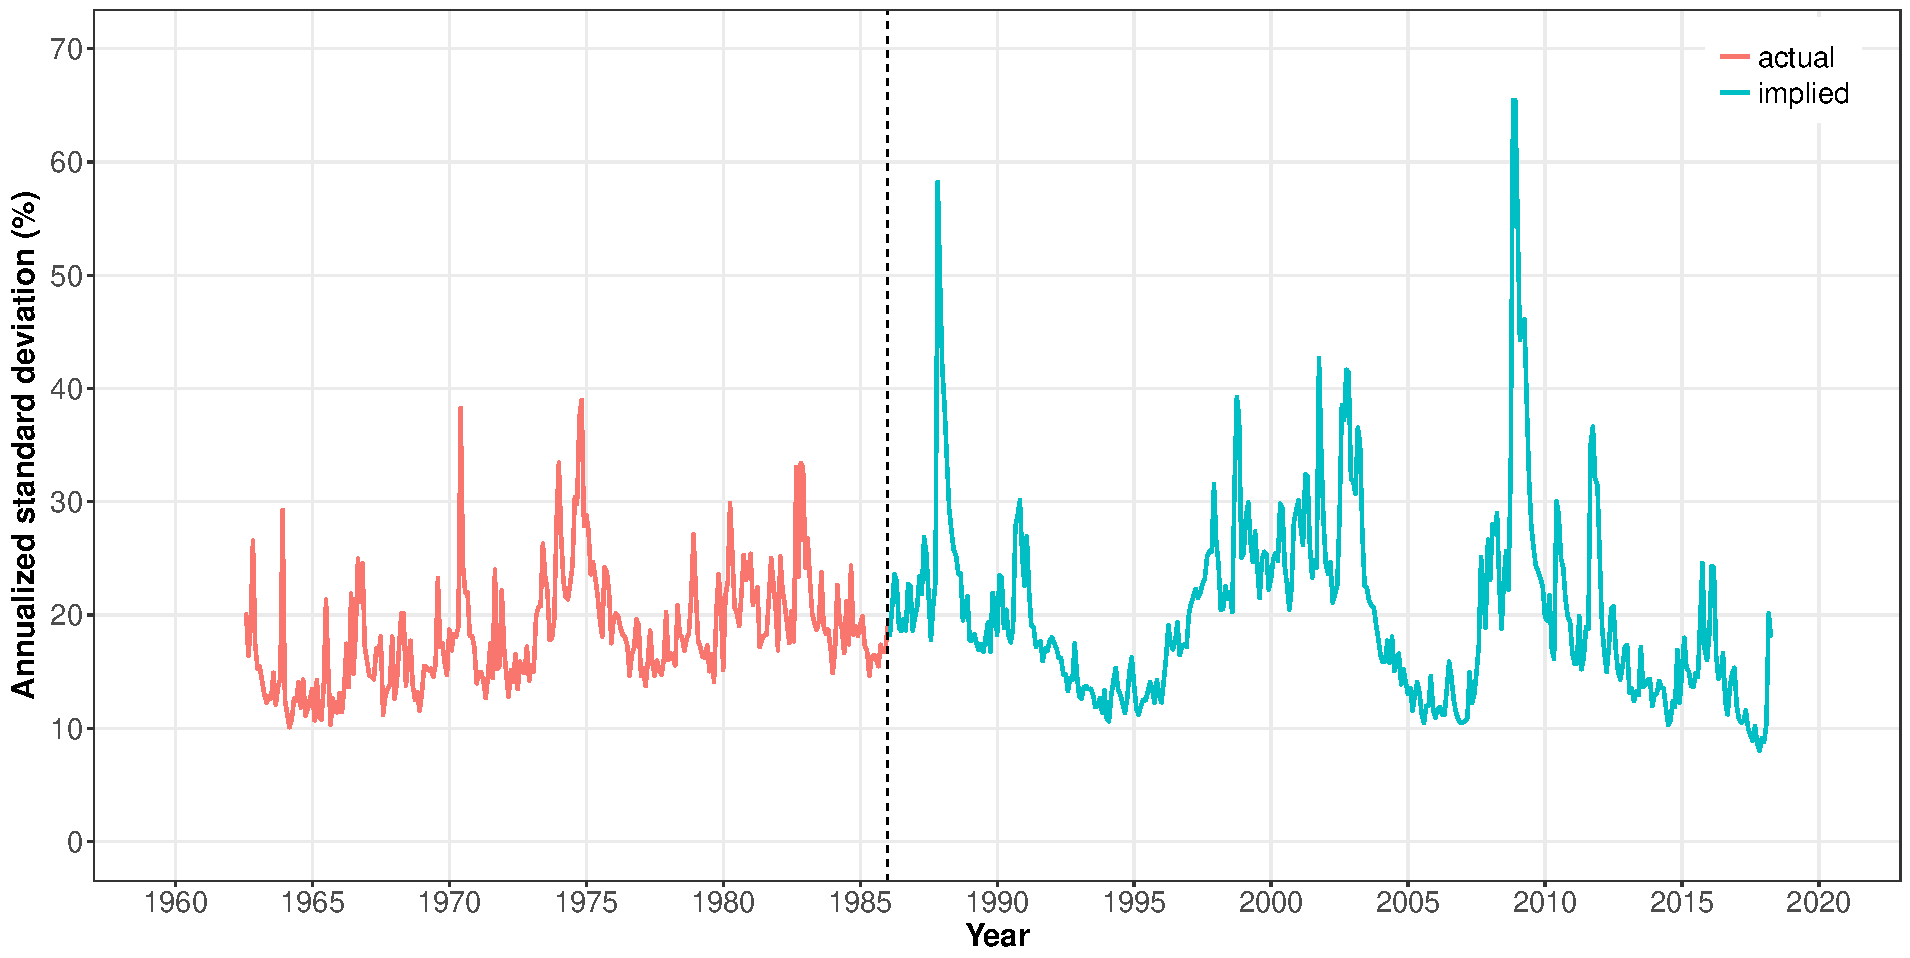
\includegraphics[trim=1cm -2.5cm 0.8cm -1cm, width=0.95\textwidth]{volatility.pdf}}
      \caption[Monthly U.S. stock market volatility.]{Monthly U.S. stock market volatility.
      \textit{Note:} From 1986 onwards CBOE VXO index of percentage implied volatility, on a hypothetical at the money S\&P100 option 30 days to expiration. Before 1986 actual monthly returns volatilities are calculated as the monthly standard deviation of the daily S\&P500 index normalized to the same mean and variance as the VXO index when they overlap from 1986 - 2003.}
   \label{fig:volatility}
\end{figure}

The derivation of the 'Bloom-shocks' (i.e., an indicator variable that takes a value of 1 for an event labelled as a 'shock') then is done as follows:
\begin{enumerate}[i]
	\item detrend the volatility-measure from above (\citet{bloom:09} uses a HP-filter with $\lambda = 129,600$); see also Figure~\ref{fig:volatility_trend} below which shows the calculated \textit{trend}-series in red. 
	\item according to \citet{bloom:09}, the actual shocks are then chosen as those events with stock-market volatility more than 1.65 standard deviations above the HP-detrended mean (selected as the 5\% one-tailed significance level) of the stock-market volatility series; thereby each month is being treated as an independent observation (see Figure~\ref{fig:volatility_cycle_shocks}; dates where the dashed line crosses the volatility-series are considered shocks)
\end{enumerate}

Ultimately, this results in identified 'shocks' as shown in Figure~\ref{fig:volatility_cycle_shocks2} which is a replication of Figure~\ref{fig:volatility_trend} but with the episodes added that correspond to the 'Bloom-shock' being equal to $1$. Correspondingly, Table~\ref{tab:bloom_shocks} spells out the exact dates.
\begin{figure}[hbt]
   \centering
   \setlength\fboxsep{0pt}
   \setlength\fboxrule{0pt}
   \fbox{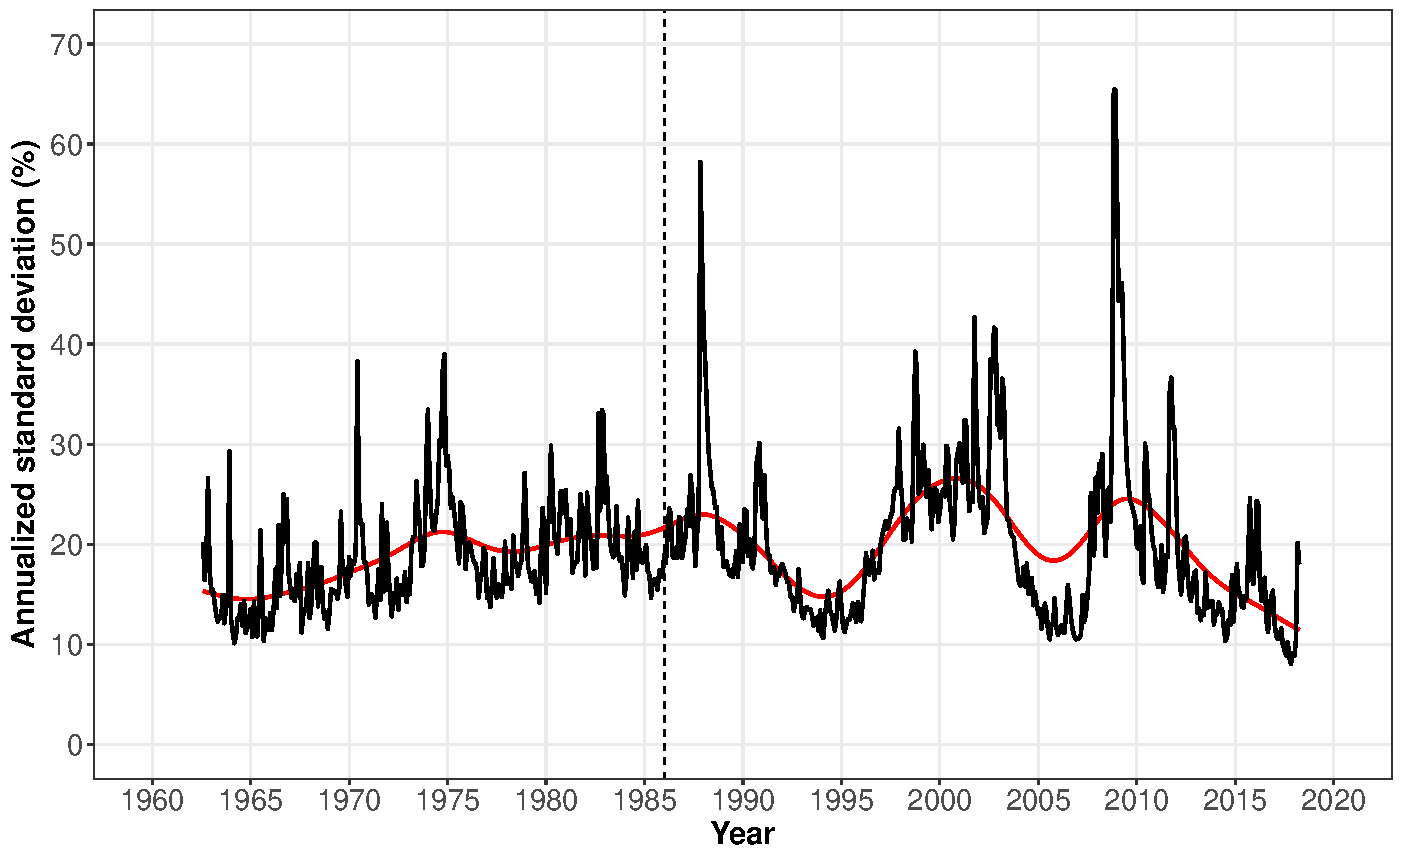
\includegraphics[trim=1cm -2.5cm 0.8cm -1cm, width=0.95\textwidth]{volatility_trend.pdf}}
      \caption[Monthly U.S. stock market volatility and HP-filtered trend.]{Monthly U.S. stock market volatility and HP-filtered trend.
      \textit{Note:} HP-filtered trend was calculated using a smoothing parameter $\lambda = 129,6000$.}   \label{fig:volatility_trend}
\end{figure}


\begin{figure}[hbt]
   \centering
   \setlength\fboxsep{0pt}
   \setlength\fboxrule{0pt}
   \fbox{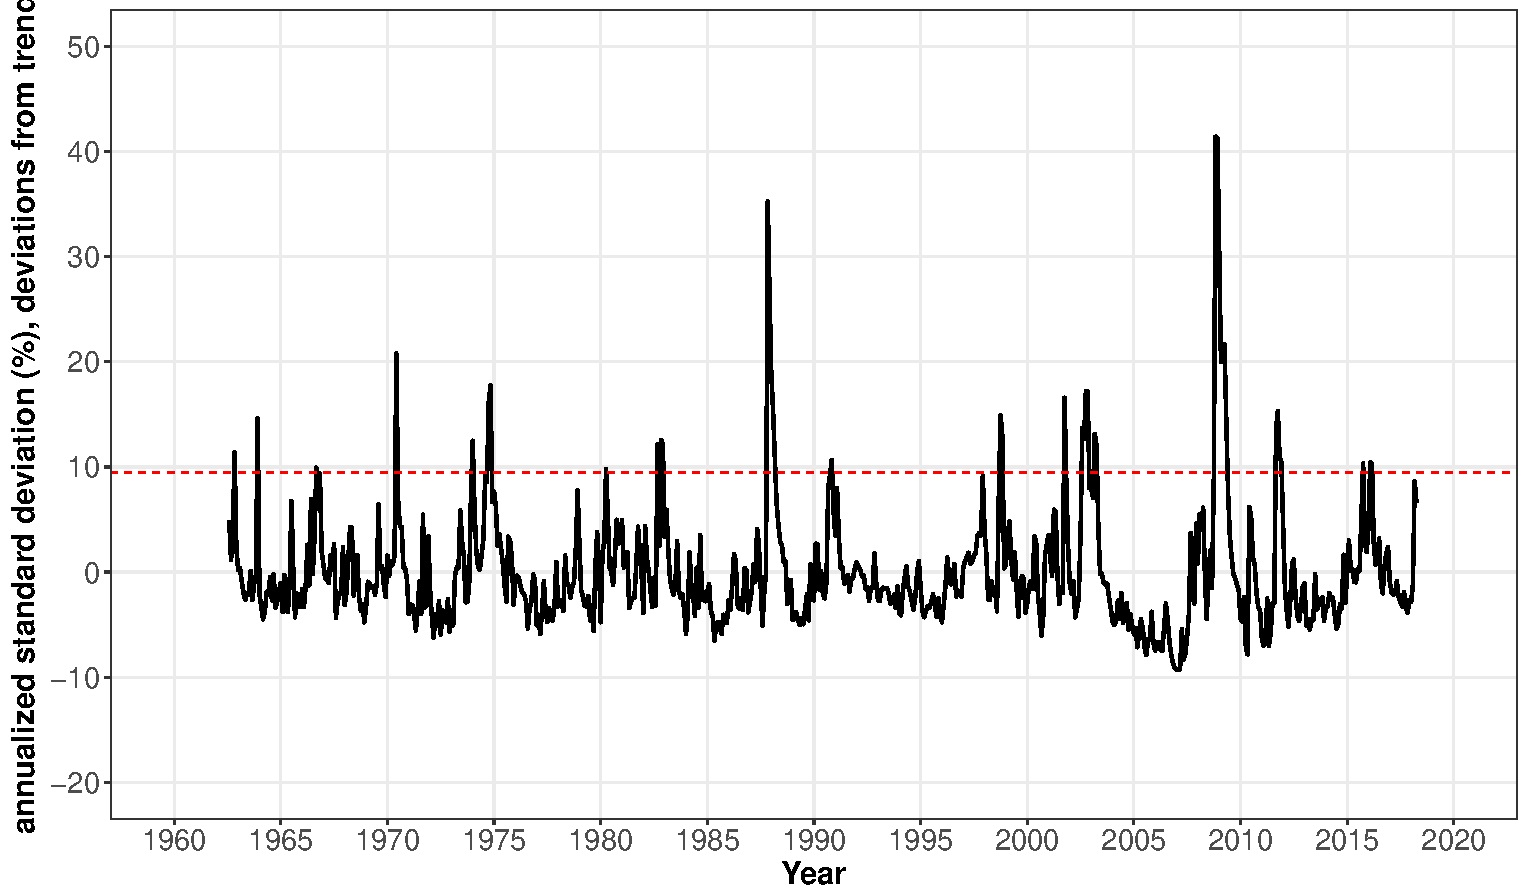
\includegraphics[trim=1cm -2.5cm 0.8cm -1cm, width=0.95\textwidth]{volatility_cycle_shocks.pdf}}
      \caption[Monthly U.S. stock market volatility and HP-filtered trend.]{Monthly U.S. stock market volatility and HP-filtered trend.
      \textit{Note:} HP-filtered trend was calculated using a smoothing parameter $\lambda = 129,6000$.}   \label{fig:volatility_cycle_shocks}
\end{figure}

\begin{figure}[hbt]
   \centering
   \setlength\fboxsep{0pt}
   \setlength\fboxrule{0pt}
   \fbox{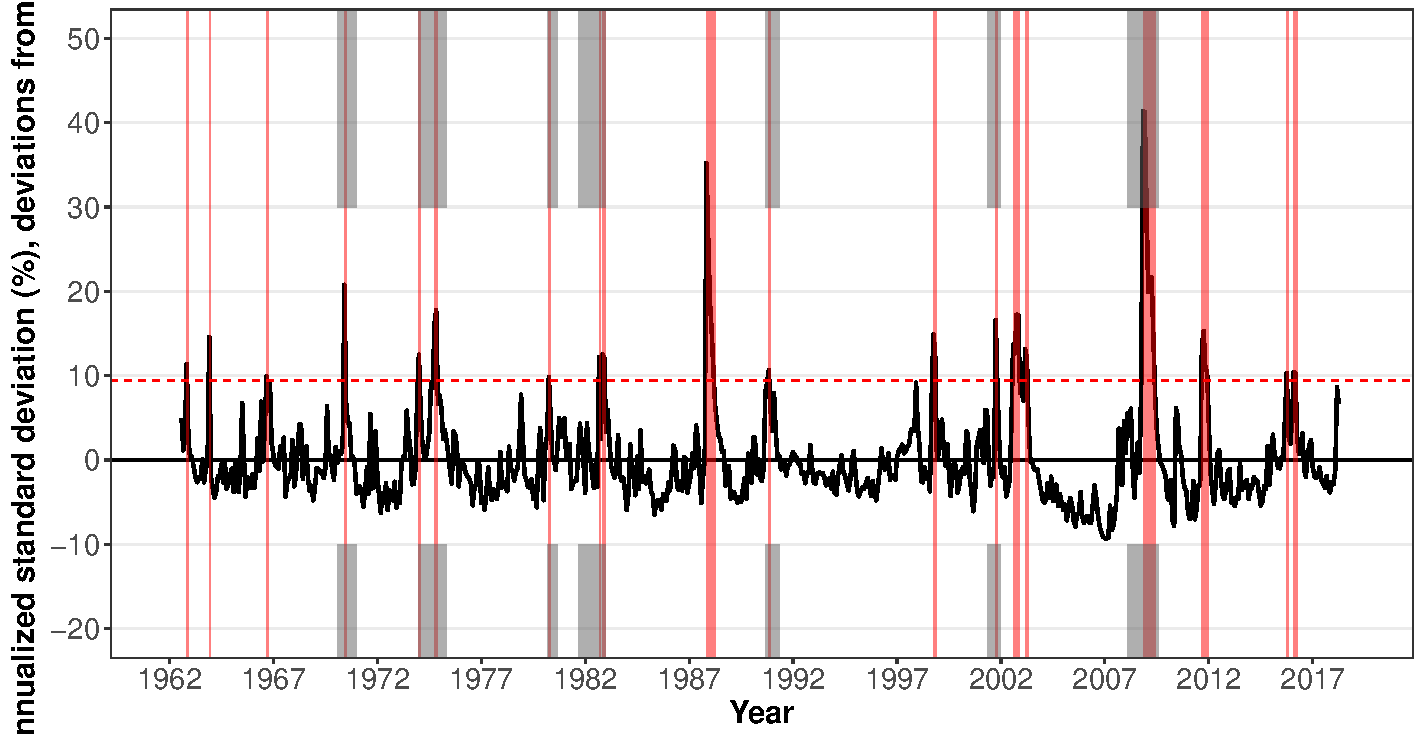
\includegraphics[trim=1cm -2.5cm 0.8cm 1cm, width=0.95\textwidth]{volatility_cycle_shocks2.pdf}}
      \caption[Monthly U.S. stock market volatility including Bloom-shocks (shaded areas).]{Monthly U.S. stock market volatility including Bloom-shocks (shaded areas).}   \label{fig:volatility_cycle_shocks2}
\end{figure}

\begin{table}[h] 
\begin{center}
\caption{Replication of shocks using Bloom's methodology.}
\scalebox{1}{
    \begin{tabular}{cccccc}
    \hline
         yearmon_start & yearmon_end & duration & yearmon_max & max_vol \\ \hline
        Nov 1962 & Nov 1962 & 1 months & Nov 1962 & 26.58\% \\
        Dec 1963 & Dec 1963 & 1 months & Dec 1963 & 29.28\% \\
        Sep 1966 & Sep 1966 & 1 months & Sep 1966 & 24.99\%\\
        Jun 1970 & Jun 1970 & 1 months & Jun 1970 & 38.27\% \\
        Jan 1974 & Jan 1974 & 1 months & Jan 1974 & 33.44\% \\
        Oct 1974 & Nov 1974 & 1 months & Nov 1974 & 38.98\% \\
        Apr 1980 & Apr 1980 & 1 months & Apr 1980 & 29.86\% \\
        Sep 1982 & Sep 1982 & 1 months & Sep 1982 & 33.05\% \\
        Nov 1982 & Dec 1982 & 2 months & Nov 1982 & 33.43\% \\
        Nov 1987 & Mar 1988 & 5 months & Nov 1987 & 58.22\% \\
        Nov 1990 & Nov 1990 & 1 months & Nov 1990 & 30.13\% \\
        Oct 1998 & Nov 1998 & 1 months & Oct 1998 & 39.25\% \\
        Oct 2001 & Oct 2001 & 1 months & Oct 2001 & 42.69\% \\
        Aug 2002 & Nov 2002 & 4 months & Oct 2002 & 41.66\% \\
        Mar 2003 & Apr 2003 & 1 months & Mar 2003 & 36.54\% \\
        Nov 2008 & May 2009 & 7 months & Nov 2008 & 65.45\% \\
        Sep 2011 & Dec 2011 & 4 months & Oct 2011 & 36.64\% \\
        Oct 2015 & Oct 2015 & 1 months & Oct 2015 & 24.60\% \\
        Feb 2016 & Mar 2016 & 2 months & Feb 2016 & 24.33\% \\
        \hline
        \hline
    \end{tabular}
}
\label{tab:bloom_shocks}
\end{center}
\end{table}




\subsection{Alternative Uncertainty-Measures}
\begin{itemize}
	\item I could potentially at some point refer to economic sentiment indicators like \url{https://www.oenb.at/en/Statistics/Standardized-Tables/\\
	Economic-and-Industry-Indicators/Economic-Indicators/Economic-Sentiment-Indicator-for-the-Euro-Area.html} or \url{https://data.europa.eu/euodp/data/dataset/c04BuUz6WXIQGJkHPwLug}.
\end{itemize}


%\newpage
\chapter{Methodology}
In his original estimations, \citet{bloom:09} estimates a range of VARs including the variables log(S\&P 500 stock market index), a stock-market volatility indicator (the 'Bloom-shocks' we have constructed above!), the Federal Funds Rate, log(average hourly earnings), log(consumer price index), hours, log(employment), and log(industrial production). Thereby all variables are HP detrended in the baseline estimations.\\
Instead, we use the \citet{jorda:05} local projection method to estimate impulse responses which estimates regressions of the dependent variables at horizon $t+h$ on the shock in period $t$ and uses the coefficient on the shock as the impulse response estimate.
\\
\\
The estimated series of regressions looks as follows:\footnote{Note an Hans: die Spezifikation wird natürlich noch überarbeitet. Ist nur eine baseline, um den code zu implementieren.}

\begin{equation} \label{eq:2.1}
z_{t+h} = \alpha_h + \theta_h shock_t + control variables + \epsilon_{t+h}
\end{equation}\\

In the above specification, $z_{t+h}$ is the variable of interest (in our case we look at industrial production and employment in manufacturing), the control variables include the log of the S\&P500 stock market index, the Federal Funds Rate and three lags of the dependent variable $z$ itself and the shock refers to the 'Bloom-shock' which we have constructed above.\footnote{All variables are HP-detrended.} For the series of regressions we look five years ahead, i.e., estimate 61 regressions using monthly data (starting to count at $h=0$). The coefficient $\theta_h$ gives the response of the dependent variable $z$ at time $t+h$ to the shock at time $t$. And because the $\epsilon_{t+h}$ will be autocorrelated, the standard errors must be HAC, i.e. \textit{hereoskedasticity and autocorrelation consistent}.\\
The data-sources are described in Appendix~\ref{sec:data}


\chapter{Results}
Figures \ref{fig:irf1} and \ref{fig:irf2} plot the preliminary responses of industrial production and employment (in manufacturing) to a shock at time $t$. \\
\\
Note to self:
\begin{itemize}
	\item as compared to \citet{bloom:09}, we already see a different pattern (BUT: we have not yet fully 'translated' the model or replicated the data-generating process that \citet{bloom:09} assumes (see next point below)
	\item bezüglich das DGP: wie sollte unsere Spezifikation aussehen um möglichst nahe an den von Bloom unterstellten DGP ranzukommen? Mit anderen Worten: Wie 'übersetzt' man einen VAR in local projections?
\end{itemize}

\begin{figure}[hbt]
   \centering
   \setlength\fboxsep{0pt}
   \setlength\fboxrule{0pt}
   \fbox{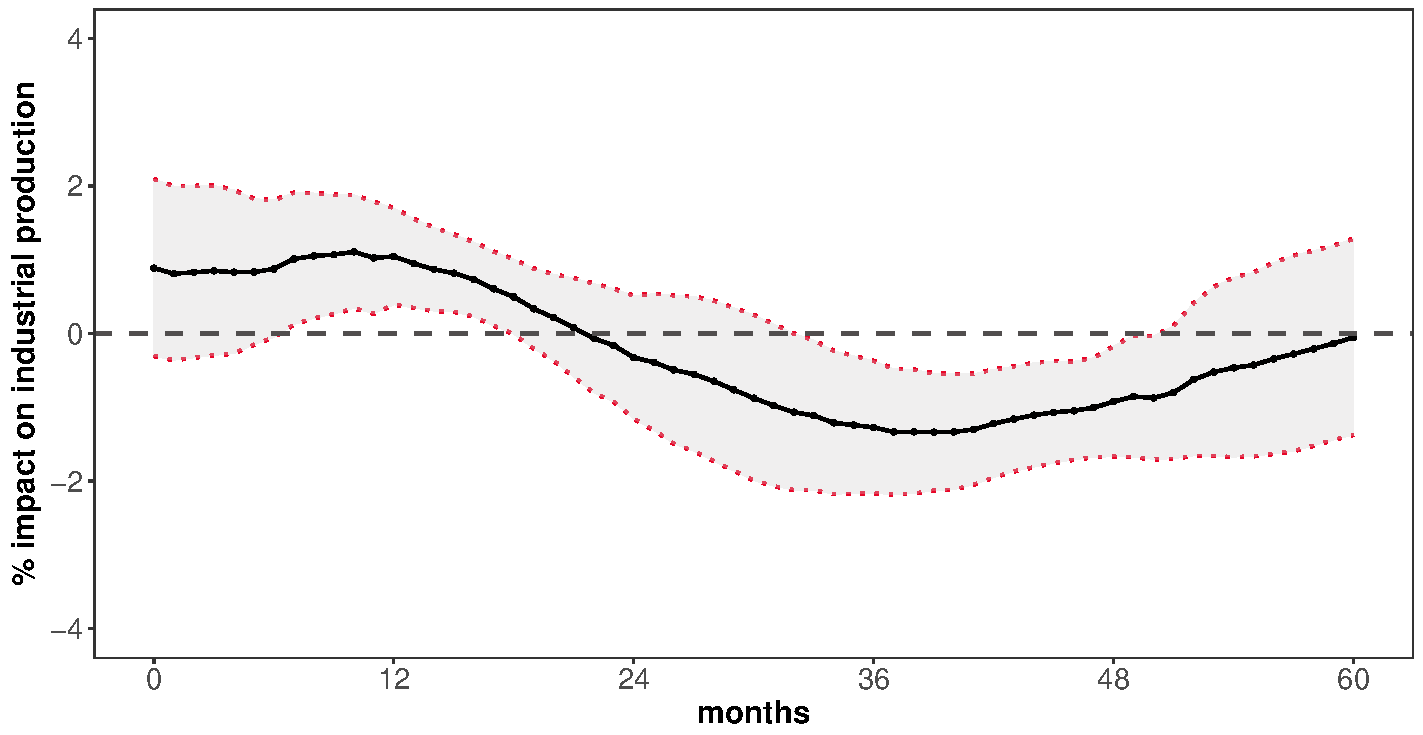
\includegraphics[trim=1cm -2.5cm 0.8cm -1cm, width=0.8\textwidth]{irf1.pdf}}
      \caption[Local projection estimations of the impact of a volatility shock on industrial production.]{Local projection estimations of the impact of a volatility shock on industrial production.
      \textit{Note:} Dashed lines are 1 standard-error bands around the response to a volatility shock.}
   \label{fig:irf1}
\end{figure}


\begin{figure}[hbt]
   \centering
   \setlength\fboxsep{0pt}
   \setlength\fboxrule{0pt}
   \fbox{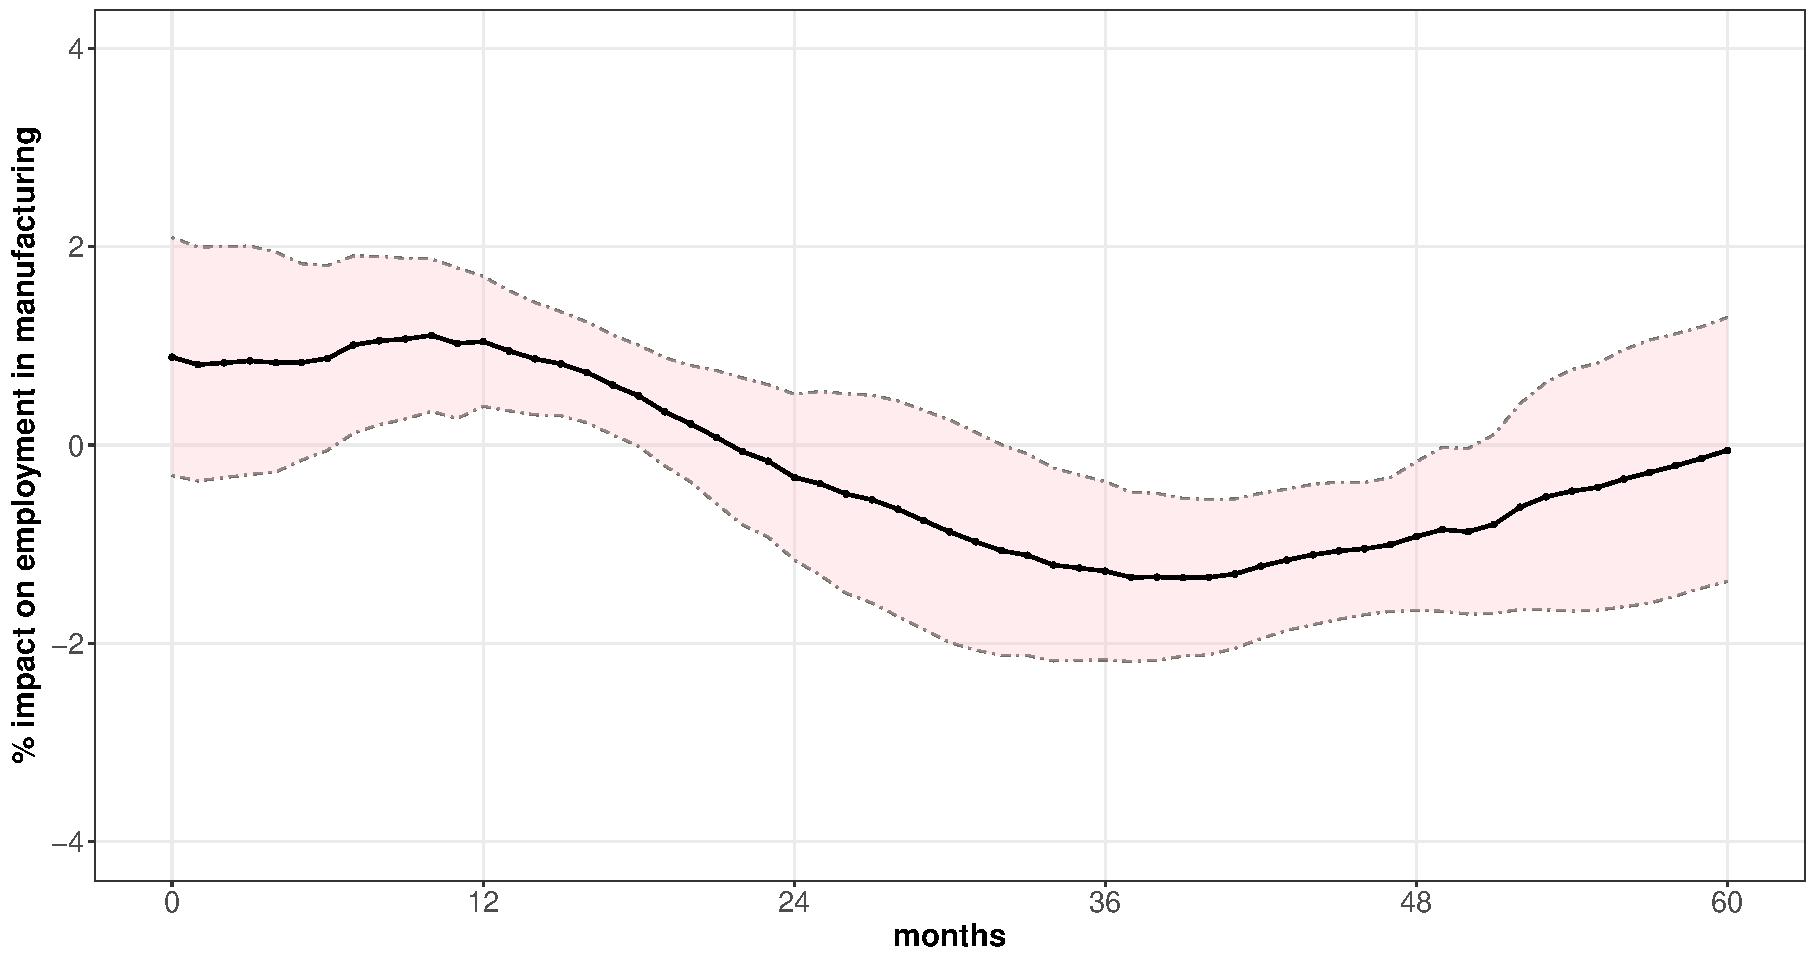
\includegraphics[trim=1cm -2.5cm 0.8cm -1cm, width=0.8\textwidth]{irf2.pdf}}
      \caption[Local projection estimations of the impact of a volatility shock on employment in manufacturing.]{Local projection estimations of the impact of a volatility shock on industrial production.
      \textit{Note:} Dashed lines are 1 standard-error bands around the response to a volatility shock.}
   \label{fig:irf2}
\end{figure}


%\newpage
\chapter{Conclusion}




%%%%%%%%%%%%%%%%%%AB HIER ENDET DER INHALT DER ARBEIT%%%%%%%%%%%%%%%%%%%%%
%%%%%%%%%%%%%%%%%%AB HIER ENDET DER INHALT DER ARBEIT%%%%%%%%%%%%%%%%%%%%%
%%%%%%%%%%%%%%%%%%AB HIER ENDET DER INHALT DER ARBEIT%%%%%%%%%%%%%%%%%%%%%
\newpage
\appendix

\chapter{Appendix}
\section{Data}
\label{sec:data}
\section{Code}
\label{sec:rcode}
%\begin{Verbatim}[fontsize=\small]
%halloe
%\end{Verbatim} 

%\begin{verbatim}
%halloe
%\end{verbatim} 

\begingroup
\fontsize{10pt}{12pt}\selectfont
\begin{verbatim}  
##The Code will go here.



\end{verbatim}  
\endgroup

\chapter{Appendix}
\section{IRFs in a VAR-Setting}
\section{IRFs and Local Projections}

%%%%%%%%%%%%%%%%%%%%%%%%%BIBLIOGRAPHY%%%%%%%%%%%%%%%%%%%%%%%%%%%%
%%%%%%%%%%%%%%%%%%%%%%%%%BIBLIOGRAPHY%%%%%%%%%%%%%%%%%%%%%%%%%%%%
%%%%%%%%%%%%%%%%%%%%%%%%%BIBLIOGRAPHY%%%%%%%%%%%%%%%%%%%%%%%%%%%%

\nocite{*}
\clearpage
\thispagestyle{empty}
\bibliographystyle{agsm}
%bibliographystyle{agsm} bewirkt, dass KEINE Beistriche zwischen den Jahreszahlen sind. Dafür aber
%Gänsefüßchen beim Titel der Werke!
\bibliography{mybiblio}





%%%%%%%%%%%%%%%%%%%%%%EIDESSTATTLICHE ERKLÄRUNG%%%%%%%%%%%%%%%%%%%%%%
\clearpage
\thispagestyle{empty}
\null\vspace{46pt}
\paragraph{\large{Eidesstattliche Erklärung}}
\vspace{43pt}
Ich erkläre hiermit an Eides Statt, dass ich die vorliegende Masterarbeit selbständig angefertigt habe. Die aus fremden Quellen direkt oder indirekt übernommenen Gedanken sind als solche kenntlich gemacht.\\
\\
Die Arbeit wurde bisher weder in gleicher noch in ähnliche Form einer anderen Prüfungsbehörde vorgelegt und auch noch nicht veröffentlicht.\\[10mm]
Innsbruck, July 2018
\begin{flushright}[htb]
     \includegraphics[trim=4cm 24.5cm 6cm 3cm, width=0.5\textwidth]{Signature.pdf}
\end{flushright}
\hspace*{256pt}
(Marcel Kropp)


%%%%%%%%%%%%%%%%%%%%%%EIDESSTATTLICHE ERKLÄRUNG%%%%%%%%%%%%%%%%%%%%%%

\end{document}
%%%%%%%%%%%%%%%%%%%%%%END OF THE DOCUMENT%%%%%%%%%%%%%%%%%%%%%%%%%%
%%%%%%%%%%%%%%%%%%%%%%END OF THE DOCUMENT%%%%%%%%%%%%%%%%%%%%%%%%%%
%%%%%%%%%%%%%%%%%%%%%%END OF THE DOCUMENT%%%%%%%%%%%%%%%%%%%%%%%%%%